\chapter{Resultados}

O trabalho ficou quatro meses adquirindo partidas da API do LOL, sendo que apenas 14 mil partidas aproximadamente eram válidas para os filtros descritos na Seção \ref{chap:aquisicao} que dizem que as partidas devem ser ranqueadas e não terem os dados incompletos.
Onde com esse algoritmo foram armazenadas \numpartidas\ jogos válidos diferentes, com esse escopo, o número de partidas usados foram ao todo \partidasrankeds\ contando com o \textit{dataset} público.
Na tabela \ref{tab:subset-lol} é possível ver uma pequena fatia dos dados salvos.


\begin{table}[H]
	\centering
	\caption{Exemplo de \textit{subset} salvo no banco de dados}
	\label{tab:subset-lol}
	\resizebox{\textwidth}{!}{%
		\begin{tabular}{cccccccccc}
			match\_id  & kills & deaths & assists & win & champ\_id & lane   & player\_id & platform & type \\
			1282000002 & 11    & 10     & 7       & 0   & 67        & BOTTOM & 16112724   & BR1      & 420  \\
			1282000002 & 2     & 8      & 15      & 0   & 412       & BOTTOM & 18604874   & BR1      & 420  \\
			1282000002 & 7     & 4      & 7       & 0   & 34        & MIDDLE & 19281809   & BR1      & 420  \\
			1282000002 & 7     & 6      & 4       & 0   & 5         & JUNGLE & 21304223   & BR1      & 420  \\
			1282000002 & 5     & 7      & 12      & 0   & 98        & TOP    & 651014     & BR1      & 420  \\
			1282000002 & 0     & 6      & 23      & 1   & 44        & BOTTOM & 18592234   & BR1      & 420  \\
			1282000002 & 19    & 5      & 5       & 1   & 222       & BOTTOM & 7170345    & BR1      & 420 
		\end{tabular}%
	}
	\small{Fonte: Autor.}
\end{table}

Com os dados armazenados, e o processamento deles executado, foi feito o \textit{webservice} que consegue exibir para o usuário informações sobre a topologia do grafo, como quem é adequado contra um campeão específico, ou com o campeão.
Na Figura \ref{fig:web_service_relatorio} é possível ver um exemplo de uso do serviço para uma visão geral das informações. Sendo que na Figura \ref{fig:topologiawebservice} mostra quem tem uma sinergia com quem (arestas verdes) e quem é um \textit{counter pick} do outro (arestas com uma seta vermelha orientando o grafo). O tamanho das arestas dos campeões indica a quantidade de vezes que que aquele determinado herói jogou com os filtros escolhidos pelo usuário.



\begin{figure}[H]
	
	\centering
	\caption{Exemplo de uso do \textit{web service} para visão geral dos dados.}
	\subfloat[Filtro dos dados para campeões da mesma equipe.]{
		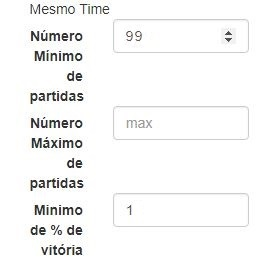
\includegraphics[width=0.4\textwidth]{imagens/web_1.JPG}
	}
	\subfloat[Filtro dos dados para adversários.]{
		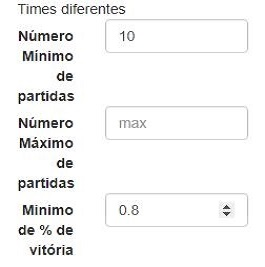
\includegraphics[width=0.4\textwidth]{imagens/web_2.JPG}
	}
	\qquad
	\subfloat[Filtro para escolher quais campeões podem participar (\textit{picks}) e quais nao podem (\textit{bans}).]{
		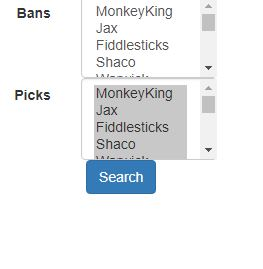
\includegraphics[width=0.4\textwidth]{imagens/web_3.JPG}
	}
	\subfloat[Exemplo de grafo exibido pelo \textit{web service}, sendo as setas vermelhas mostrando quem é bom contra quem, e as linhas continuas quem é bom com quem. O tamanho do circulo é a frequência daquela ligação e a cor é a força da ligação.]{
		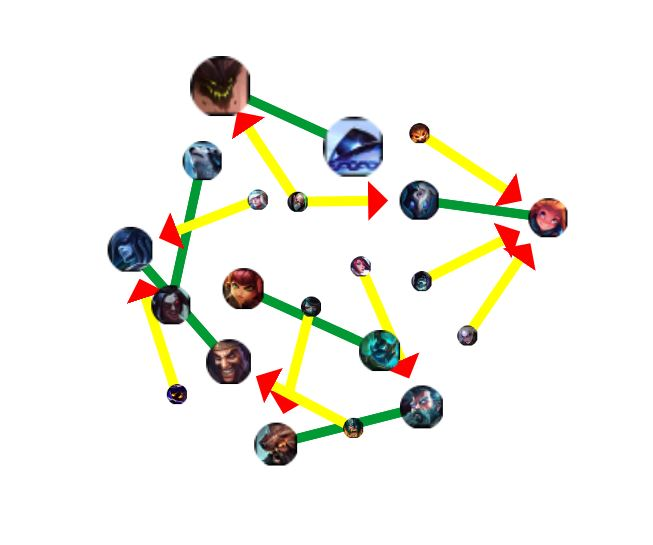
\includegraphics[width=0.4\textwidth]{imagens/web_4.JPG}
		\label{fig:topologiawebservice}
	}
	
	\small{Fonte: Autor.}
	\label{fig:web_service_relatorio}
\end{figure}


É possível ver topologia da rede complexa final na Figura \ref{fig:cnfinal}, que consta com 139 vértices diferentes ( todos os heróis lançados até a aquisição dos dados ) e com 19180 arestas já que estas são orientadas.

\begin{figure}[H]
	\caption{Visualização da topologia final da Rede Complexa.}
	\begin{center}
		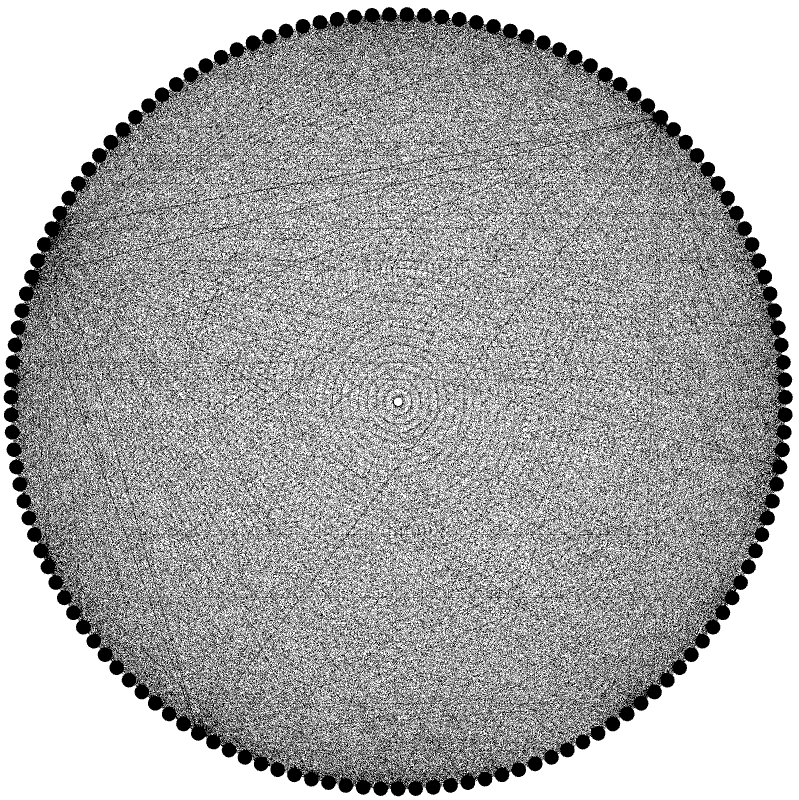
\includegraphics[width=1\textwidth]{imagens/grafofinal.png}
	\end{center}
	\small{Fonte: Autor.}
	\label{fig:cnfinal}
\end{figure}

\begin{figure}[H]
	\caption{Erro do KNN em variação ao K.}
	\begin{center}
		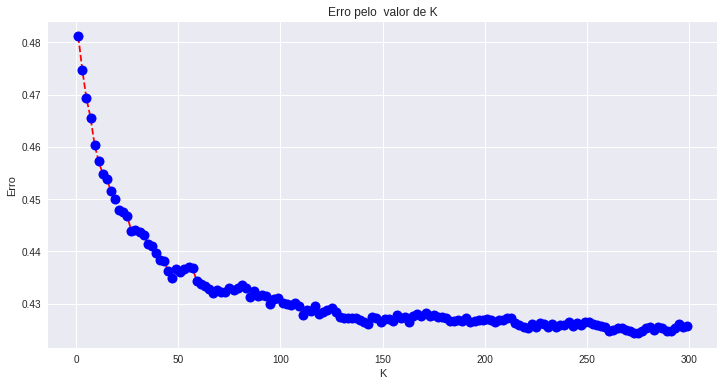
\includegraphics[width=1\textwidth]{imagens/knn.png}
	\end{center}
	\small{Fonte: Autor.}
	\label{fig:KNNgrafico}
\end{figure}


O Classificador KNN ficou com uma precisão de 58\% com a melhor calibração conseguida, com o \(k = 243\), na Figura \ref{fig:KNNgrafico} é possível ver a precisão em relação ao \(k\). E com o modelo preparado é possível entrar no \textit{webservice} e selecionar os campeões de cada time e conferir o resultado da predição. É possível ver um exemplo de uso do \textit{webservice} na Figura \ref{fig:predicaowebservice} onde possível ver a sinergia dos dois times e a entropia da partida.

Com a matriz de confusão é possível ver as classificações corretas e as erradas por resultado, ou seja, na Tabela \ref{tab:confusion} é possível ver quantas vezes o KNN classificou sendo vencedor o time 0, porém era vencedor o time 1 ou qualquer outro cenário.

\begin{table}[]
	\centering
	\caption{Matriz de confusão do KNN}
	\label{tab:confusion}
		\resizebox{\textwidth}{!}{%
\begin{tabular}{|c|c|c|}
	\hline
	Real x Predição & time 0 & time 1 \\ \hline
	time 0          & 10909  & 6993   \\ \hline
	time 1          & 7848   & 9107   \\ \hline
\end{tabular}
}
\
\
\small{Fonte: Autor.}
\end{table}


\begin{figure}[H]
	
	\centering
	\caption{Exemplo de uso do \textit{webservice} predição da partida}
	\subfloat[Área para escolher o time 0.]{
		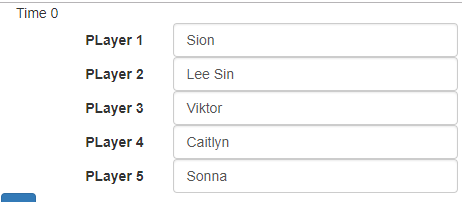
\includegraphics[width=0.4\textwidth]{imagens/predict_1.PNG}
	}
	\subfloat[Área para escolher o time 1.]{
		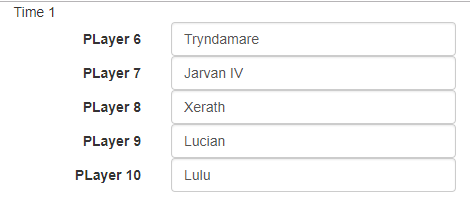
\includegraphics[width=0.4\textwidth]{imagens/predict_2.PNG}
	}
	\qquad
	\subfloat[Exemplo de resposta do \textit{webservice}.]{
		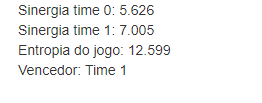
\includegraphics[width=0.4\textwidth]{imagens/predict_3.PNG}
	}
	\subfloat[Tela toda da parte de predição.]{
		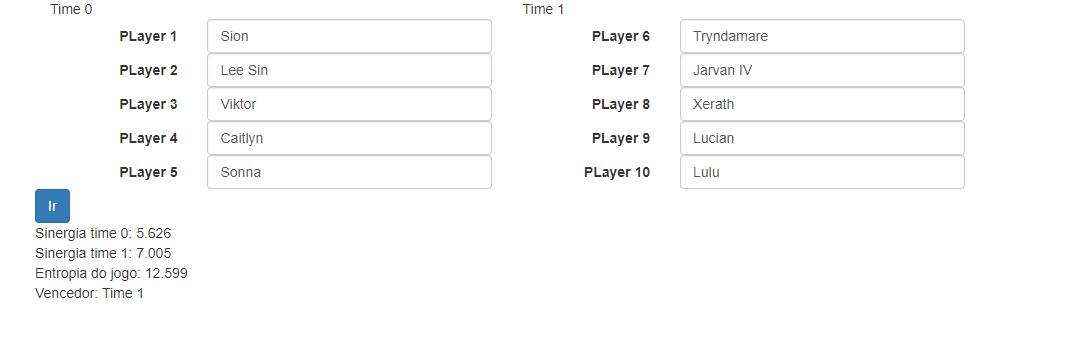
\includegraphics[width=0.4\textwidth]{imagens/predict_4.PNG}
	}
	
	
	\small{Fonte: Autor.}
	\label{fig:predicaowebservice}
\end{figure}
\